\documentclass[a4paper]{scrartcl}
\usepackage[utf8]{inputenc}
\usepackage[english]{babel}
\usepackage{graphicx}
\usepackage{lastpage}
\usepackage{pgf}
\usepackage{wrapfig}
\usepackage{fancyvrb}
\usepackage{fancyhdr}
\pagestyle{fancy}
\usepackage{minted}


% Create header and footer
\headheight 27pt
\pagestyle{fancyplain}
\lhead{\footnotesize{Data Storage Paradigms, IV1351}}
\chead{\footnotesize{Project Report}}
\rhead{}
\lfoot{}
\cfoot{\thepage\ (\pageref{LastPage})}
\rfoot{}

\title{Project Report}
\subtitle{Data Storage Paradigms, IV1351}
\author{}
\date{Date: 17-11-2026}

\begin{document}

\maketitle
\noindent\textbf{Project members:} \\ \hfill
[Arvin Emrani, emrani@kth.se] \\ \hfill
[Hugo Johansson, hujo@kth.se] \\ \hfill
[Matilda Sköldin, mskoldin@kth.se] \\ \hfill

\section*{Declaration:}

By submitting this assignment, it is hereby declared that all group members listed above have contributed to the solution. It is also declared that all project members fully understand all parts of the final solution and can explain it upon request.

It is furthermore declared that the solution below is a contribution by the project members only, and specifically that no part of the solution has been copied from any other source (except for lecture slides at the course IV1351), no part of the solution has been provided by someone not listed as a project member above, and no part of the solution has been generated by a system.

\section*{Tips for Report Writing}
\textbf{REMOVE THIS SECTION BEFORE SUBMITTING THE REPORT.}\\

\noindent \textit{The target audience has exactly the same skills as the author, except they do not know anything at all about the specific application described in the report.} \\

Consider the following:

\begin{itemize}
  \item \textbf{The report must be \textit{centered around the requirements}. Which are they (Introduction), how did you work to meet them (Method), what is the solution that meets them (Result), and how can you be sure they are met (Discussion). This is the IMRaD method.} The requirements on the Introduction, Method, Result and Discussion chapters are described below under each chapter.

  \item Is spelling and grammar correct? Is spoken language avoided?

  \item Does the report have a good structure with sections, subsections and paragraphs?

  \item Is the text clarified with images and/or other figures, and with links to the code in your Git repository? Remember that all figures (images, tables, graphs, code listings, etc) shall be numbered and have a short explaining text.
\end{itemize}

\section{Introduction}

\textbf{This chapter tells \textit{what} are you going to do.} 

\textbf{Explain the task and the requirements on the solution. It's important to clearly state the requirements. \textit{Also specify which other student you worked with when solving the tasks, or if you worked alone.} }

The task is to design and implement a database, where the conceptual model given in the instructions is the basis for the database. The objective is to create a logical and physical model, that stores the data described in the instructions, without including any unnecessary information. The attributes, entities and relations described in the conceptual model must be a part of the final logical model. The logical model should be normalized and then used to create an actual database. Another requirement includes generating data for the finished database, to demonstrate that the database functions properly.

The group worked independently for every part of the task except for the trigger, which was done in collaboration with another student during tutorial, the name of the other student is unfortunately unknown. 


\section{Literature Study}
 
\textbf{(This chapter must prove that you collected sufficient knowledge before starting development, instead of just hacking away without knowing how to complete a task. State what you have read and briefly summarize what you have learned.)}

Before the start of the project the videolectures on the "conceptual model" and "logical to physical model" were watched to understand how to use the program Astah and how to create the logical model. The takeaway from the lectures was that there were 11 steps to create the logical model. Briefly the 11 steps include creating entities, normalising the tables, how to consider the constraints of foreign keys and many-to-many relations.

The lecture regarding normalisation was also attended before staring the work. This lecture gave a good understanding as how to normalize the model to get an efficient and well-structured database. 1NF ensures that all attributes are atomic and that there isn't any multi-valued attributes. 2NF removes partial dependencies by ensuring that all non-key attributes depend on the primary key. 3NF removes transative dependencies, by ensuring that non-key attributes depend only on candidate keys.  

The document "tips and tricks for seminar 1" was also read before the start of the project. This gave useful insight on how to create surrogate keys, generate data, multivalued attributes and how to handle relations to one self.  

\section{Method}

\textbf{This chapter tells} \textit{how} you solved the task.
\textbf{
Explain how you worked when solving the tasks and how you evaluated that your solution met the requirements. \textit{Do not explain your solution and do not refer to code}, that belongs to the \textit{Result} chapter. More specific instructions for the content can be found under each task on the Project page in Canvas.}

First of all, the conceptual model was analyzed and compared to the assignment description to get an understanding of how the relations were derived. After that, the lecture "logical to physical models" was used as a frame to translate the given conceptual model to a logical and physical model, using the program Astah. 

Tables were created for each entity. The tables included columns for each attribute, which also specified a data-type.  Column constraints had to be carefully considered, i.e assigning NOT NULL requirements to attributes that are required to have a value, and also identifying which attributes that had to have an unique value. Thereafter, the model had to be normalized. The attributes were carefully inspected to find multi-valued attributes and assigning them separate tables, to make the model 1NF.

To create the database the logical model was exported to SQL code in Astah. The constraints which were comments in the logical model where translated to SQL code manually.

The creation of the trigger was done in collaboration with another student during the tutorial, it was done manually in visual studio code, with help on the tutorial and the postgres documentation. 

To generate data for the database the AI-program Claude was used. To create the the data our create database SQL-code was inserted into Claude along with the relevant parts from the description of the assignment. 

First the database was made in pgAdmin and then the create\_database query was executed, then the trigger query was executed and at last the data was inserted.

To confirm that data was inserted correctly some test where preformed. The command select * was used on all the tables to see that no data was corrupted or wrong. Some joins between tables where also tested. During the execution of the tests an inspection of the foreign keys was preformed to ensure that they were correct. The trigger was also tested by trying to insert a course instance extra to the same employee that already had 4 instances the same period. 

\section{Result}

\textbf{This chapter explains \textit{the result} of what you did.}

\textbf{The report must show that you have done the work yourself and that you have understood what you have done, both of these goals are met by carefully explaining your solution here in the result chapter, and proving that it meets the requirements. \textit{State each requirement that is met} and explain \textit{how you met it}. Also include links to your code in your Git repository, and include also diagrams, see Figure \ref{fig:diag}, and other figures to illustrate your reasoning. All figures must be referenced in the text. Ask yourself if the solution is clearly explained, and if the reader will understand the application. What would you yourself want to know if you read about the application, is that included in the report? More specific instructions for the content can be found under each task on the Project page in Canvas. }

The logical model that was created can be seen in figure \ref{fig:placeholder}. It has all the entities, attributes and relations defined in the conceptual model. In the model the red rectangles are comments, and they specify when an attribute is unique and foreign key constraints. All of the strong entities have a surrogate key which was created with INT GENERATED ALWAYS IDENTITY, which function as primary keys. For multi-valued attributes separate tables have been created, for example teaching\_activity has a separate table and is referenced with an id. The employee\_table has a relation to itself to enable that every employee has a supervisor, which is also an employee. The employee\_skill\_set table is a many-to-may relation and therefore has a crosstable, where every employee is able to have multiple skills. 

\begin{figure}
    \centering
    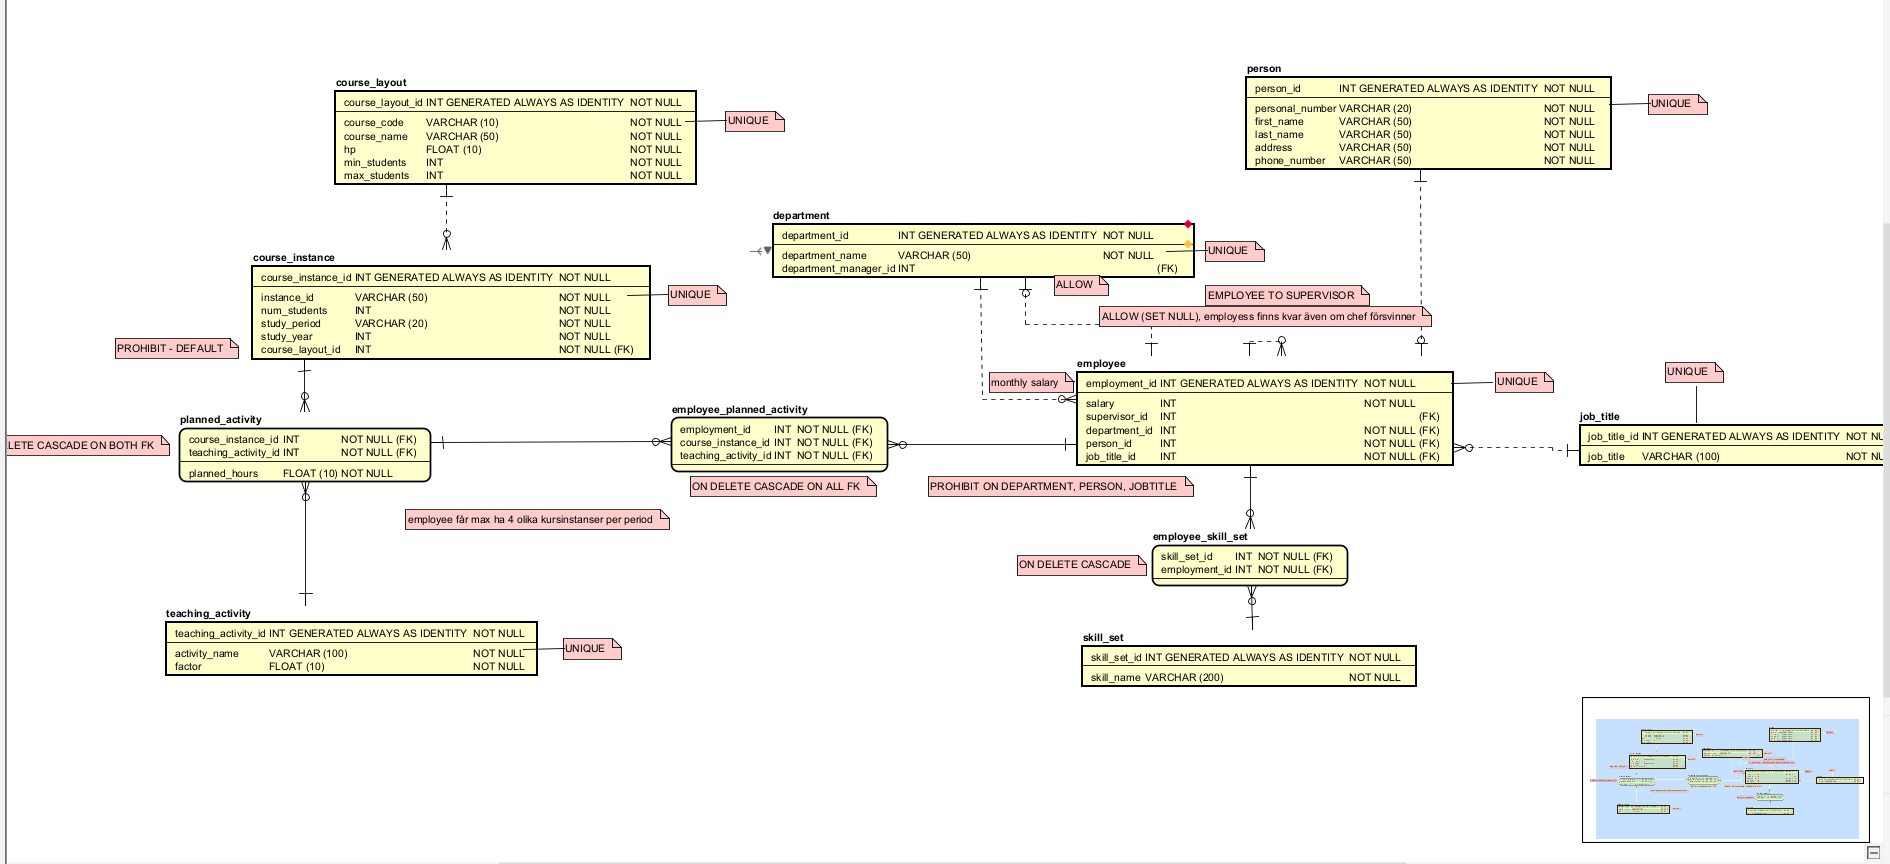
\includegraphics[width=0.5\linewidth]{Skärmbild 2026-11-18 103053.png}
    \caption{The created logical model}
    \label{fig:placeholder}
\end{figure}

The code to create our database can be found here.

To verify that the database works as intended, the business overview in the project description was analyzed to see that the given information and data could be retrieved from the database throguh different operations. Several queries were used to verify that the necessary data could be fetched. The logical model gave a clear overview as of which tables are connected. Perhaps the most important operation to verify is that joining tables can be performed correctly. For example, by running the query:


\begin{minted}{sql}
SELECT * FROM course_layout AS c
JOIN course_instance AS d
ON c.course_layout_id = d.course_layout_id
\end{minted}

One could verify that all courses could be identified with it's instances including the other attributes from the tables. A lot of other queries were used to retrieve data from the database and obviously not all of them can be listed in this report. The query above was just given as a simple example to demonstrate a bit of the process in verifying the correctness of the database.

Another important result is to verify is that the trigger-function actually works. One requirement of the assignment was that each teacher could teach maximum 4 course instances simultaneously during a single period. The trigger was therefore designed to execute before whenever an employee is assigned an course instance. Whenever a fifth course instance was tried to be assigned to an employee, the trigger raised an exception an printed a message stating that it was not possible. Therefore the trigger worked exactly as intended.  




\section{Discussion}

\textbf{This chapter \textit{analysis} the result presented in the previous section.} 

E\textbf{valuate your solution according to the assessment criteria found in the assessment-criteria documents, which are found under the bullet \textit{In the Discussion chapter of your report...}, under each task on the Project page in Canvas. You do not have to cover all specified criteria.}

The naming conventions are followed according to the video "logical and physical models". The crow foot notation is correctly 

\section{Comments About the Course}

\textbf{This section is optional, but please at least write approximately how much time you spent on the assignment, including lectures, labs, tutorials and seminars. This is of great help for course evaluation.

Also, any other comment(s) related to this course offering or to coming offerings is much appreciated. }




\end{document}

